\chapter{Étape 7 — Construire les guides imprimables}
\label{chap:guides}

\begin{chapeau}
Cette étape transforme la prescription en deux pièces à imprimer : un \textbf{guide de coupe}, qui guide la scie et
les broches, et un \textbf{guide de réduction}, qui tient les fragments dans la position corrigée pendant la fixation.
Chaque pièce est ensuite vérifiée par des contrôles indépendants de sa construction.
\end{chapeau}

\begin{figure}[htbp]
\centering
\tikz\node[fill=grisfond, rounded corners=6pt, inner xsep=10pt, inner ysep=10pt]{%
  \panneau{8.3cm}{rendu_face.png}{a}{face d'appui}\hspace{12pt}%
  \panneau{8.3cm}{rendu_profil.png}{b}{profil}\hspace{12pt}%
  \panneau{8.3cm}{rendu_reduction.png}{c}{guide de réduction}\hspace{12pt}%
  \panneau{8.3cm}{rendu_fermeture.png}{d}{coin de fermeture}};
\caption{Les guides construits par le logiciel sur un tibia (os fictif). (a) à (c) : coin d'ouverture posé par la
face médiale. (a) Le guide de coupe vu de sa face d'appui (bleu : moitié proximale ; vert : moitié distale ; orange :
ponts sécables). (b) Le profil, avec les broches. (c) Après la coupe et la correction : les broches sont parallèles et
le guide de réduction (violet) s'y enfile jusqu'à l'os corrigé. (d) Le guide de coupe d'un coin de fermeture : deux
moitiés, la partie au-dessus du coin osseux appartient à la moitié distale ; la fibula, qui passerait devant le guide
dans cette vue, n'est pas dessinée.}
\label{fig:guide-v3}
\end{figure}

\section{Ce que l'on construit}

Le \textbf{guide de coupe} est une \textbf{coque} moulée sur l'os, qui ne s'emboîte que dans une seule position.
Elle porte :
\begin{itemize}
  \item une \textbf{tour} par trait de coupe, percée d'une \textbf{fente} de 0,8~mm (lame de 0,6~mm et 0,2~mm de jeu)
  exactement dans le plan prescrit : une fente pour un coin d'ouverture, deux pour un coin de fermeture ;
  \item des \textbf{manchons}, un par broche (une par fragment), percés à 1,8~mm pour des broches de
  1,6~mm ;
  \item deux \textbf{ponts sécables}, petits morceaux de 2 × 5~mm aux deux bouts de la première fente, qui relient les
  deux moitiés et que l'on coupe à la pince après la coupe de l'os.
\end{itemize}

Les broches distales ne sont pas parallèles aux broches proximales avant la correction (\cref{sec:broches}). Le guide
de coupe est donc fait de deux moitiés : chacune sort en glissant le long de \emph{sa} broche. Après la correction, les deux broches sont parallèles : le \textbf{guide de réduction}, une barre à
deux manchons parallèles, s'enfile alors sur elles (\cref{sec:reduction}).

\begin{pourquoi}
\textbf{Pourquoi deux pièces simples ?} La version précédente du guide (octobre 2026) réglait aussi la profondeur de
coupe par la hauteur des tours (une graduation de lame gravée sur les tours) et transformait ses deux moitiés en verrou
de réduction (des oreilles percées d'un trou commun dans la seule position corrigée). Ces fonctions ajoutaient des
pièces, des réglages et des étapes au bloc opératoire, pour un gain qui restait à prouver sur un vrai os. Le
06/11/2026, nous avons choisi de revenir à un guide de coupe et un guide de réduction simples, le système le plus
utilisé dans les publications (\cref{chap:etat}) : moins de pièces à imprimer, un mode opératoire de 9 ou 10 étapes au
lieu de 12 à 15, et un code plus court (2\,032 lignes au lieu de 2\,827).
\end{pourquoi}

\section{Le principe : la modélisation implicite}
\label{sec:implicite}

Un solide peut être décrit par une fonction $F$ définie dans tout l'espace : $F(\vb{x}) < 0$ à l'intérieur,
$F(\vb{x}) > 0$ à l'extérieur, et la surface est $F = 0$. Si $F$ est une distance signée, les opérations de
construction deviennent de simples calculs :
\begin{equation}
  \text{union} : \min(F_1, F_2), \qquad
  \text{intersection} : \max(F_1, F_2), \qquad
  \text{différence} : \max(F_1, -F_2).
\end{equation}
Cette approche a deux avantages : elle ne casse jamais (pas de surfaces qui se croisent mal), et elle permet
d'imposer des contraintes partout dans l'espace, par exemple « pas de matière à moins de 0,3~mm de l'os ». Les champs
sont calculés sur une grille régulière de pas 0,3~mm, alignée sur la direction de pose du guide (au plus 12 millions de
nœuds ; au-delà, le pas grandit). La \cref{fig:construction} résume la construction.

\fig{construction_guide.pdf}{Les étapes de la construction des guides.}{fig:construction}

\subsection{Les formes de base}

Chaque pièce est une forme simple dont la distance signée est connue :
\begin{itemize}
  \item un \textbf{pavé} de centre $\vb{c}$, d'axes $\vb{a}_i$ et de demi-côtés $h_i$ :
  $F = \max_i \bigl(\abs{(\vb{x} - \vb{c})\cdot\vb{a}_i} - h_i\bigr)$ ; un pavé aux arêtes arrondies de rayon $r$ :
  avec $q_i = \abs{(\vb{x} - \vb{c})\cdot\vb{a}_i} - (h_i - r)$,
  \begin{equation}
    F = \norm{\max(\vb{q}, \vb{0})} + \min\bigl(\max_i q_i,\ 0\bigr) - r ;
  \end{equation}
  \item un \textbf{cylindre} d'axe $(\vb{a}, \vb{o})$, de rayon $R$, entre les abscisses $t_0$ et $t_1$ : avec
  $t = (\vb{x} - \vb{a})\cdot\vb{o}$ et $\rho$ la distance à l'axe,
  $F = \max\bigl(\rho - R,\ t_0 - t,\ t - t_1\bigr)$ ;
  \item une \textbf{capsule} (un « bras ») autour du segment $[\vb{a}, \vb{b}]$ : la distance au segment moins le rayon ;
  \item un \textbf{secteur} : le dièdre d'angle $\pm A$ autour d'une direction, qui limite la coque autour de la face
  d'appui.
\end{itemize}

\subsection{L'union lisse}

Une union par $\min$ laisse des angles vifs entre la coque et les tours, qui concentrent les contraintes et
favorisent les fissures. On utilise un \textbf{minimum lisse} \cite{quilez2013} :
\begin{equation}
  \tcbhighmath{h = \clamp\!\left(\frac12 + \frac{b - a}{2k},\ 0,\ 1\right), \qquad
  \smin(a, b, k) = b + (a - b)\,h - k\,h\,(1 - h).}
\end{equation}
Loin du raccord ($\abs{a - b} > k$), $\smin = \min(a, b)$ ; près du raccord, la fonction s'arrondit et crée un congé de
rayon voisin de $k$ (0,8~mm par défaut, \cref{fig:smin}).

\fig{union_lisse.pdf}{Union nette et union lisse d'un disque et d'un pavé ; à droite, le minimum lisse le long d'une
droite.}{fig:smin}

\section{La distance à l'os}
\label{sec:distance}

Le champ de base est la distance signée $d(\vb{x})$ du nœud $\vb{x}$ à la surface de l'os, négative dans l'os
(\cref{fig:champ-distance}). Elle est calculée en trois parties :
\begin{itemize}
  \item \textbf{le signe} : chaque nœud est-il dans l'os ? On le sait par une voxelisation par rayons (règle de
  parité : un rayon qui part d'un point intérieur croise la surface un nombre impair de fois) ;
  \item \textbf{la valeur exacte près de l'os}, là où le guide peut exister : la distance au triangle le plus proche.
  Pour chaque nœud, on cherche avec un arbre k-d les six échantillons de surface les plus proches, on lit leurs
  triangles, et on calcule la distance exacte point--triangle par les régions de Voronoï du triangle (sommets, arêtes,
  face) \cite{ericson2005} ;
  \item \textbf{une valeur approchée loin de l'os}, par la transformée de distance de Maurer \cite{maurer2003}, exacte au
  voxel près et rapide.
\end{itemize}

\fig{champ_distance.pdf}{Sur une coupe transverse du tibia du lévrier : la distance signée à l'os, la coque posée par
la face médiale (abord usuel), puis par la face latérale, où l'espace entre le tibia et la fibula est
interdit.}{fig:champ-distance}

\section{La coque}

La coque est la couche d'épaisseur $e = 3$~mm posée à $j = 0{,}3$~mm de l'os :
\begin{equation}
  \tcbhighmath{j \;\leq\; d(\vb{x}) \;\leq\; j + e.}
\end{equation}
Elle est limitée :
\begin{itemize}
  \item à un secteur de $\pm 75\degre$ autour de la face d'appui, pour chaque moitié autour de son propre axe ;
  \item en longueur, à 8~mm au-delà des broches extrêmes, mais jamais à moins de 10~mm des extrémités articulaires ;
  \item près du cartilage : elle s'arrête à $j + e + 1$~mm de ses sommets ; elle ne repose jamais sur une surface
  articulaire.
\end{itemize}

\begin{attention}[title={Un jeu exact, au centième de millimètre}]
La surface finale est interpolée linéairement entre les nœuds de la grille. Sur un os convexe, elle peut passer
jusqu'à 0,03~mm trop près de l'os. Le logiciel vise donc $d \geq j + 0{,}04$~mm. Après la construction, chaque sommet
encore trop proche est repoussé le long de la normale à l'os jusqu'à $j + 0{,}005$~mm (au plus 0,15~mm), sans changer
la topologie. Le jeu mesuré sur les guides est de 0,30 à 0,33~mm.
\end{attention}

\section{Les fentes, les tours et la profondeur de coupe}
\label{sec:butee}

\subsection{Les tours}

Chaque tour est un pavé aux arêtes arrondies, centré sur un plan de coupe, avec trois axes : $\vb{n}$ (la normale du
plan), $\vb{h}$ (vers la face d'appui, d'où entre la lame) et $\vb{l}$ (le long de la fente). Sa longueur est la largeur
de l'os dans le plan de coupe, plus 1~mm et une paroi de 2~mm de chaque côté. La fente est taillée exactement dans le
plan prescrit. Le haut de la tour est à la hauteur de guidage $g = 10$~mm au-dessus de la coque, au point le plus haut
de l'os dans le plan de la fente :
\begin{equation}
  h_{\text{haut}} = h_{\max} + j + e + g.
\end{equation}

\begin{exemple}
La lame a 0,2~mm de jeu dans sa fente et elle est guidée sur au moins 13~mm au-dessus de l'os : son inclinaison est
au plus $\arctan(0{,}2/13) \approx 0{,}9\degre$. Les entrées des fentes et des manchons sont chanfreinées (0,5~mm à
45\degre) pour que la lame et les broches entrent sans accrocher.
\end{exemple}

\subsection{La profondeur de coupe}

Le danger d'une coupe guidée est d'aller trop loin et de casser la charnière. Chaque fente a un \textbf{arrêt} : la
charnière (coupe incomplète), ou la corticale opposée (coupe complète, que la lame traverse). On note $h_{\text{stop}}$
sa hauteur le long de $\vb{h}$. Quand la charnière est presque dans le plan de coupe (moins de 30\degre), la fente lui
est rendue \textbf{parallèle} : la lame, enfoncée perpendiculairement au haut de la tour, atteint la charnière à la même
profondeur sur toute la longueur de la fente. Le logiciel calcule cette \textbf{profondeur de lame}
(\cref{fig:profondeur}) :
\begin{equation}
  D = h_{\text{haut}} - h_{\text{stop}},
\end{equation}
et la donne au chirurgien dans le mode opératoire, sur le plan coté et dans l'application, au dixième de millimètre :
il la repère sur sa lame. Pour le coin d'ouverture de la \cref{fig:guide-v3}, $D = 24{,}5$~mm.

\fig{profondeur_lame.pdf}{La profondeur de lame $D$ : du haut de la tour à la charnière (a), ou à la corticale
opposée en coupe complète (b).}{fig:profondeur}

\section{Les manchons}

Chaque manchon est un cylindre de rayon $0{,}9 + 2 = 2{,}9$~mm autour de l'axe de sa broche, de l'os jusqu'à
$j + e + g = 13{,}3$~mm au-dessus de lui (ou moins si la planification l'a raccourci, jamais moins de $j + e + 4$~mm).
Le trou de 1,8~mm est percé par une opération booléenne exacte, coaxial à la broche prescrite. Si le cartilage ou un os
voisin coupe la coque et isole un manchon, un \textbf{bras} (une capsule du rayon du manchon) le relie au haut de la
tour de sa moitié, par-dessus l'os et hors du trajet de la lame.

\section{Les contraintes dures}
\label{sec:contraintes-dures}

Les contraintes forment un champ $G$, et le solide final est $\{\max(F, G) < 0\}$ : là où $G > 0$, aucune matière n'est
possible.

\textbf{Le jeu.} $G \geq (j + 0{,}04) - d$ : jamais de matière à moins du jeu de l'os ; de même, au moins 1~mm de tout
os voisin (fibula, rotule, fabelles), dont la distance est calculée sur une petite grille autour de chacun.

\textbf{Pas de contre-dépouille.} Le guide se pose en translation, par la face d'appui, et chaque moitié sort en
glissant le long de ses broches. Aucune matière ne doit donc se trouver « sous » l'os, vu depuis ces directions
(\cref{fig:depouille}). Pour une direction $\vb{g}$, on calcule la \emph{carte de hauteur} de l'os : pour chaque colonne
parallèle à $\vb{g}$, la hauteur maximale de l'os,
\begin{equation}
  H(\vb{x}_\perp) = \max_{\vb{p}\,\in\,\text{os},\ \vb{p}_\perp = \vb{x}_\perp} \vb{p}\cdot\vb{g}.
\end{equation}
On la « dilate » ensuite par une fonction qui ajoute le jeu (des calottes de rayon $j$) et un \textbf{cône de
dépouille} de demi-angle $\alpha = 5\degre$ :
\begin{equation}
  H'(\vb{x}_\perp) = \max_{\vb{y}_\perp}\Bigl[H(\vb{y}_\perp) + S\bigl(\norm{\vb{x}_\perp - \vb{y}_\perp}\bigr)\Bigr],
  \qquad
  S(\rho) = \begin{cases} \sqrt{j^2 - \rho^2} & \rho \leq j, \\ -(\rho - j)/\tan\alpha & \rho > j. \end{cases}
\end{equation}
Un point est interdit s'il est sous cette enveloppe : $\vb{x}\cdot\vb{g} < H'(\vb{x}_\perp) - 0{,}5$~mm (la tolérance de
0,5~mm laisse le jeu exact commander sur la face visible). La contrainte est appliquée pour la pose du guide entier,
puis pour le retrait de chaque moitié. Les os voisins entrent aussi dans les cartes de hauteur.

\fig{depouille.pdf}{Une coque qui embrasse l'os au-delà de sa silhouette ne peut être ni posée ni retirée ; la
contrainte de dépouille l'arrête à la silhouette.}{fig:depouille}

\textbf{L'espace entre les os.} Entre le tibia et la fibula, il y a la membrane interosseuse et des muscles : on ne
peut ni y glisser une pièce, ni y forer, ni y faire sortir la lame. Tranche par tranche le long de l'os, l'espace
interdit est ce que l'enveloppe convexe de l'os \emph{et} du voisin ajoute à l'enveloppe convexe de l'os seul
(\cref{fig:champ-distance}, à droite). Les creux de l'os lui-même restent couverts par la coque.

\begin{attention}[title={Une erreur corrigée grâce au chirurgien}]
Jusqu'au 22/10/2026, un guide de tibia pouvait être posé du côté de la fibula : il passait tous les contrôles
géométriques (jeu, dépouille, retrait), mais il était impossible à poser. Depuis, cet espace est interdit, et un coin
dont la lame devrait passer par là est refusé avec une explication. Pour toute nouvelle pièce, il faut se demander
comment le chirurgien la pose, la fixe et coupe à travers.
\end{attention}

\textbf{Le cartilage.} Aucune partie du guide (tours et manchons compris) à moins de 1,5~mm des sommets de cartilage.

\textbf{Les parties trop fines.} Une lèvre de moins de 1,2~mm casserait à l'impression. Une \emph{ouverture
morphologique} (érosion puis dilatation) par une boule de 0,6~mm de rayon retire ces parties, sans toucher aux surfaces
exactes.

\section{De la grille au solide exact}

Le champ final est converti en surface par Flying Edges (comme au \cref{chap:maillage}), puis en un solide
\emph{manifold} : chaque arête appartient à exactement deux triangles. Toutes les découpes fines sont ensuite faites
par des \textbf{opérations booléennes exactes} (bibliothèque manifold3d \cite{manifold}), indépendantes de la grille :
\begin{itemize}
  \item les fentes (pavés exacts), les trous des broches (cylindres) et leurs chanfreins (troncs de cône) ;
  \item la \textbf{séparation} des moitiés : une dalle de l'épaisseur de la première fente, moins les deux ponts.
\end{itemize}
Le STL est enfin relu comme le ferait un logiciel d'impression, pour vérifier qu'il est étanche ; deux sommets
confondus d'un même solide sont écartés de 2~µm si besoin.

\section{Les deux moitiés et les ponts}

La première fente sépare le guide en \textbf{deux moitiés} sur toute sa hauteur, sauf aux deux ponts. Pour un coin de
fermeture, la deuxième fente est une fente fermée de la moitié distale : la partie du guide posée sur le coin osseux
appartient à cette moitié. Après la coupe, on coupe les deux ponts ; la moitié qui s'éloigne de l'autre en glissant sur
ses broches sort la première (en fermeture la distale, en ouverture la proximale), puis l'autre ; en fermeture, on
retire ensuite le coin d'os.

\section{Le guide de réduction}
\label{sec:reduction}

\subsection{Le principe}

Après la coupe et la correction, toutes les broches sont parallèles. Le guide de réduction est une \textbf{barre}
(l'enveloppe convexe des broches vue le long des broches, épaissie du rayon des manchons), au moins 4~mm au-dessus de
l'os corrigé et des os voisins corrigés, et deux \textbf{manchons parallèles} de 12~mm qui s'appuient sur l'os corrigé
(\cref{fig:guide-v3}, image c). Il ne s'enfile sur les broches que si elles sont parallèles, jusqu'au contact de l'os ;
il bloque alors les six degrés de liberté des fragments pendant la pose de la plaque.

\subsection{Le trait de scie compensé}

Le guide de réduction est construit sur l'os \emph{corrigé}. En fermeture, chaque trait de scie enlève l'épaisseur de
la lame $s$ (0,6~mm). Quand le chirurgien ferme le coin jusqu'au contact des surfaces d'os, le fragment distal avance
encore de $s$ le long de la normale $\vb{n}_1$ du premier plan. La position réelle est donc
\begin{equation}
  \mt{T} = (\mt{R}, \vb{t})
  \quad\longrightarrow\quad
  \mt{T}_{\text{réel}} = (\mt{R},\ \vb{t} - s\,\vb{n}_1).
\end{equation}
Sans cette compensation, un guide ajusté au dixième de millimètre ne s'enfilerait pas sur les broches.

\section{Les contrôles indépendants}

Chaque guide est vérifié par des mesures qui n'utilisent pas les calculs de sa construction (\cref{tab:controles}).
Une alerte « NE PAS IMPRIMER » est donnée si un contrôle essentiel échoue.

\begin{table}[htbp]
\centering\small
\caption{Les contrôles faits sur chaque guide (fichier \fichier{guide.json}).}
\label{tab:controles}
\begin{tabularx}{\linewidth}{L{4.2cm}Y}
\toprule
\titrecol{Contrôle} & \titrecol{Méthode} \\
\midrule
jeu minimal guide--os & distance exacte de chaque sommet du guide aux triangles de l'os \\
pas d'interpénétration & volume de l'intersection exacte guide $\cap$ os (doit être nul) \\
appui & surface du guide à moins de $j + 0{,}15$~mm de l'os, pour le guide et pour chaque moitié \\
nombre de pièces & deux moitiés après la coupe des ponts, aucune pièce utile détachée \\
retrait sans heurter l'os & lancer de rayons le long des broches, depuis 4000 points de chaque moitié \\
retrait sans heurter l'autre moitié & la moitié glissée de 0,25 à 30~mm ; moins de 0,5~mm³ de recouvrement = frottement \\
manchons & matière présente dans la couronne de chaque manchon ; broches hors du trajet de la lame \\
voisins et cartilage & distances du guide, des broches et des manchons aux os voisins et au cartilage \\
profondeur de lame & calculée pour chaque fente, du haut de la tour à la charnière ou à la corticale opposée \\
guide de réduction & barre à au moins 4~mm de l'os corrigé, manchons parallèles, jeu avec l'os corrigé et les voisins \\
fichiers & STL relus : étanches et orientés \\
\bottomrule
\end{tabularx}
\end{table}

\section{Les plans 2D}

Le logiciel dessine aussi deux plans, présentés comme des \textbf{plans de pièce industrielle} (comme ceux d'AutoCAD),
en SVG, PDF et PNG :
\begin{itemize}
  \item le \textbf{plan générique} : le guide en schéma de principe, ses cotes en symboles ($j$, $e$, $g$, $p$,
  $s$\ldots) et le tableau des paramètres, avec les formules des dimensions qui découlent de l'os
  (\cref{fig:plan-generique}) ;
  \item le \textbf{plan coté du cas} : le guide construit pour cet os (\cref{fig:plan-guide}). La vue de face A est
  prise depuis la face d'appui ; la vue de gauche B est à sa droite et la vue de dessus C en dessous (projection
  européenne : les vues sont alignées et gardent les mêmes cotes). La coupe E-E passe par les manchons : elle montre
  les trous des broches, les fentes et la profondeur de lame de chaque fente, du haut de la tour jusqu'à l'arrêt de la
  lame. La vue D montre le guide de réduction le long des broches, avec l'entraxe des broches. Une vue isométrique aide
  à se représenter la pièce.
\end{itemize}
Les deux plans suivent les règles du dessin technique (normes ISO) : feuille A3 avec cadre et repères de zones,
cartouche avec le logo de l'ECAM, le numéro du plan, l'échelle et le symbole de la projection européenne, nomenclature
des pièces (les deux moitiés, les ponts, le guide de réduction, les broches) reliée aux vues par des repères numérotés ;
traits forts pour les arêtes, fins pour les cotes, mixtes pour les axes des broches et les plans de coupe de l'os ;
cotes avec flèches pleines ; surfaces coupées hachurées. L'os est montré en gris, comme une pièce voisine. L'échelle
(2:1, 1:1 ou 1:2) est la plus grande qui fait tout tenir sur la feuille ; une cote de contrôle de 50~mm permet de
vérifier l'échelle à l'impression.

Les parties cachées sont éliminées par un \textbf{tampon de profondeur} (\emph{z-buffer}) écrit en numpy : chaque pixel
garde le triangle le plus proche ; seules les arêtes de silhouette et les arêtes vives visibles sont tracées en
vecteurs. La coupe E-E est exacte : les pièces sont coupées par le plan avec manifold3d (\code{trim_by_plane},
\code{slice}).

\section{Le mode opératoire}
\label{sec:protocole}

Le logiciel écrit le mode opératoire de chaque cas dans \fichier{guide.json}, sur le plan coté, et l'affiche à
l'étape 12 (\cref{fig:deroule}) :
\begin{enumerate}
  \item abord : exposer la face d'appui de l'os sur toute la longueur du guide ;
  \item poser le guide de coupe (il ne s'emboîte que dans une seule position), puis forer les broches proximales et les
  distales à travers leurs manchons ;
  \item couper par chaque fente jusqu'à la profondeur de lame indiquée (charnière, ou corticale opposée) ; en coupe
  complète, protéger les tissus de l'autre côté (écarteur de Hohmann) ;
  \item couper les deux ponts à la pince coupe-broche ;
  \item retirer la moitié indiquée en premier, puis l'autre, et le coin d'os en fermeture ;
  \item si la fibula croise le plan de coupe tibial, l'ostéotomiser : intacte, elle empêcherait la correction ;
  \item fermer (ou ouvrir) le coin et, s'il le faut, tourner le fragment distal, jusqu'à ce que toutes les broches
  soient parallèles ;
  \item enfiler le guide de réduction sur les broches jusqu'au contact de l'os ;
  \item fixer (plaque), puis retirer le guide de réduction et les broches.
\end{enumerate}

\fig{deroule_operation.pdf}{Le déroulé prévu d'une opération avec les deux guides. Ce déroulé n'a pas encore été
essayé.}{fig:deroule}

\section{Un guide paramétrique}

Le guide est un \textbf{modèle paramétrique}, comme une pièce de CAO pilotée par une table : 22 dimensions de
conception (jeu, épaisseur, lame, broches, ponts, guide de réduction\ldots) se règlent dans l'application, dans des
bornes de sécurité ; leurs valeurs par défaut sont dans \fichier{parametres.py} (\cref{ann:parametres}). Toutes les
autres dimensions découlent de l'os : longueur des fentes, hauteur des tours, étendue de la coque, position des
broches. Un nouveau scanner donne donc un nouveau guide, construit avec les mêmes règles.

\begin{danslecode}
\fichier{code_source/etape7_guide.py} : \code{generer()} (point d'entrée), \code{verifier_abord()} (refus motivé),
\code{guide_coupe()} (grille, champs, contraintes, isosurface, booléens, moitiés), \code{Grille},
\code{distance_signee()}, \code{DistanceSurface} et \code{dist2_point_triangle()} (distance exacte), \code{smin()},
\code{champ_boite_arrondie()}, \code{champ_cylindre()}, \code{champ_capsule()}, \code{champ_secteur()},
\code{carte_hauteur()}, \code{depouille()}, \code{ombre()}, \code{EntreOs}, \code{sans_parties_fines()},
\code{isosurface()}, \code{transformation_reelle()}, \code{os_corrige()}, \code{guide_reduction()},
\code{controles_coupe()}, \code{controles_reduction()}, \code{protocole()}, \code{assurer_jeu()}. Les plans 2D sont
dessinés par \fichier{code_source/dessin_guide.py}.
\end{danslecode}

\begin{landscape}
\pagestyle{paysage}
\begin{figure}[p]
\centering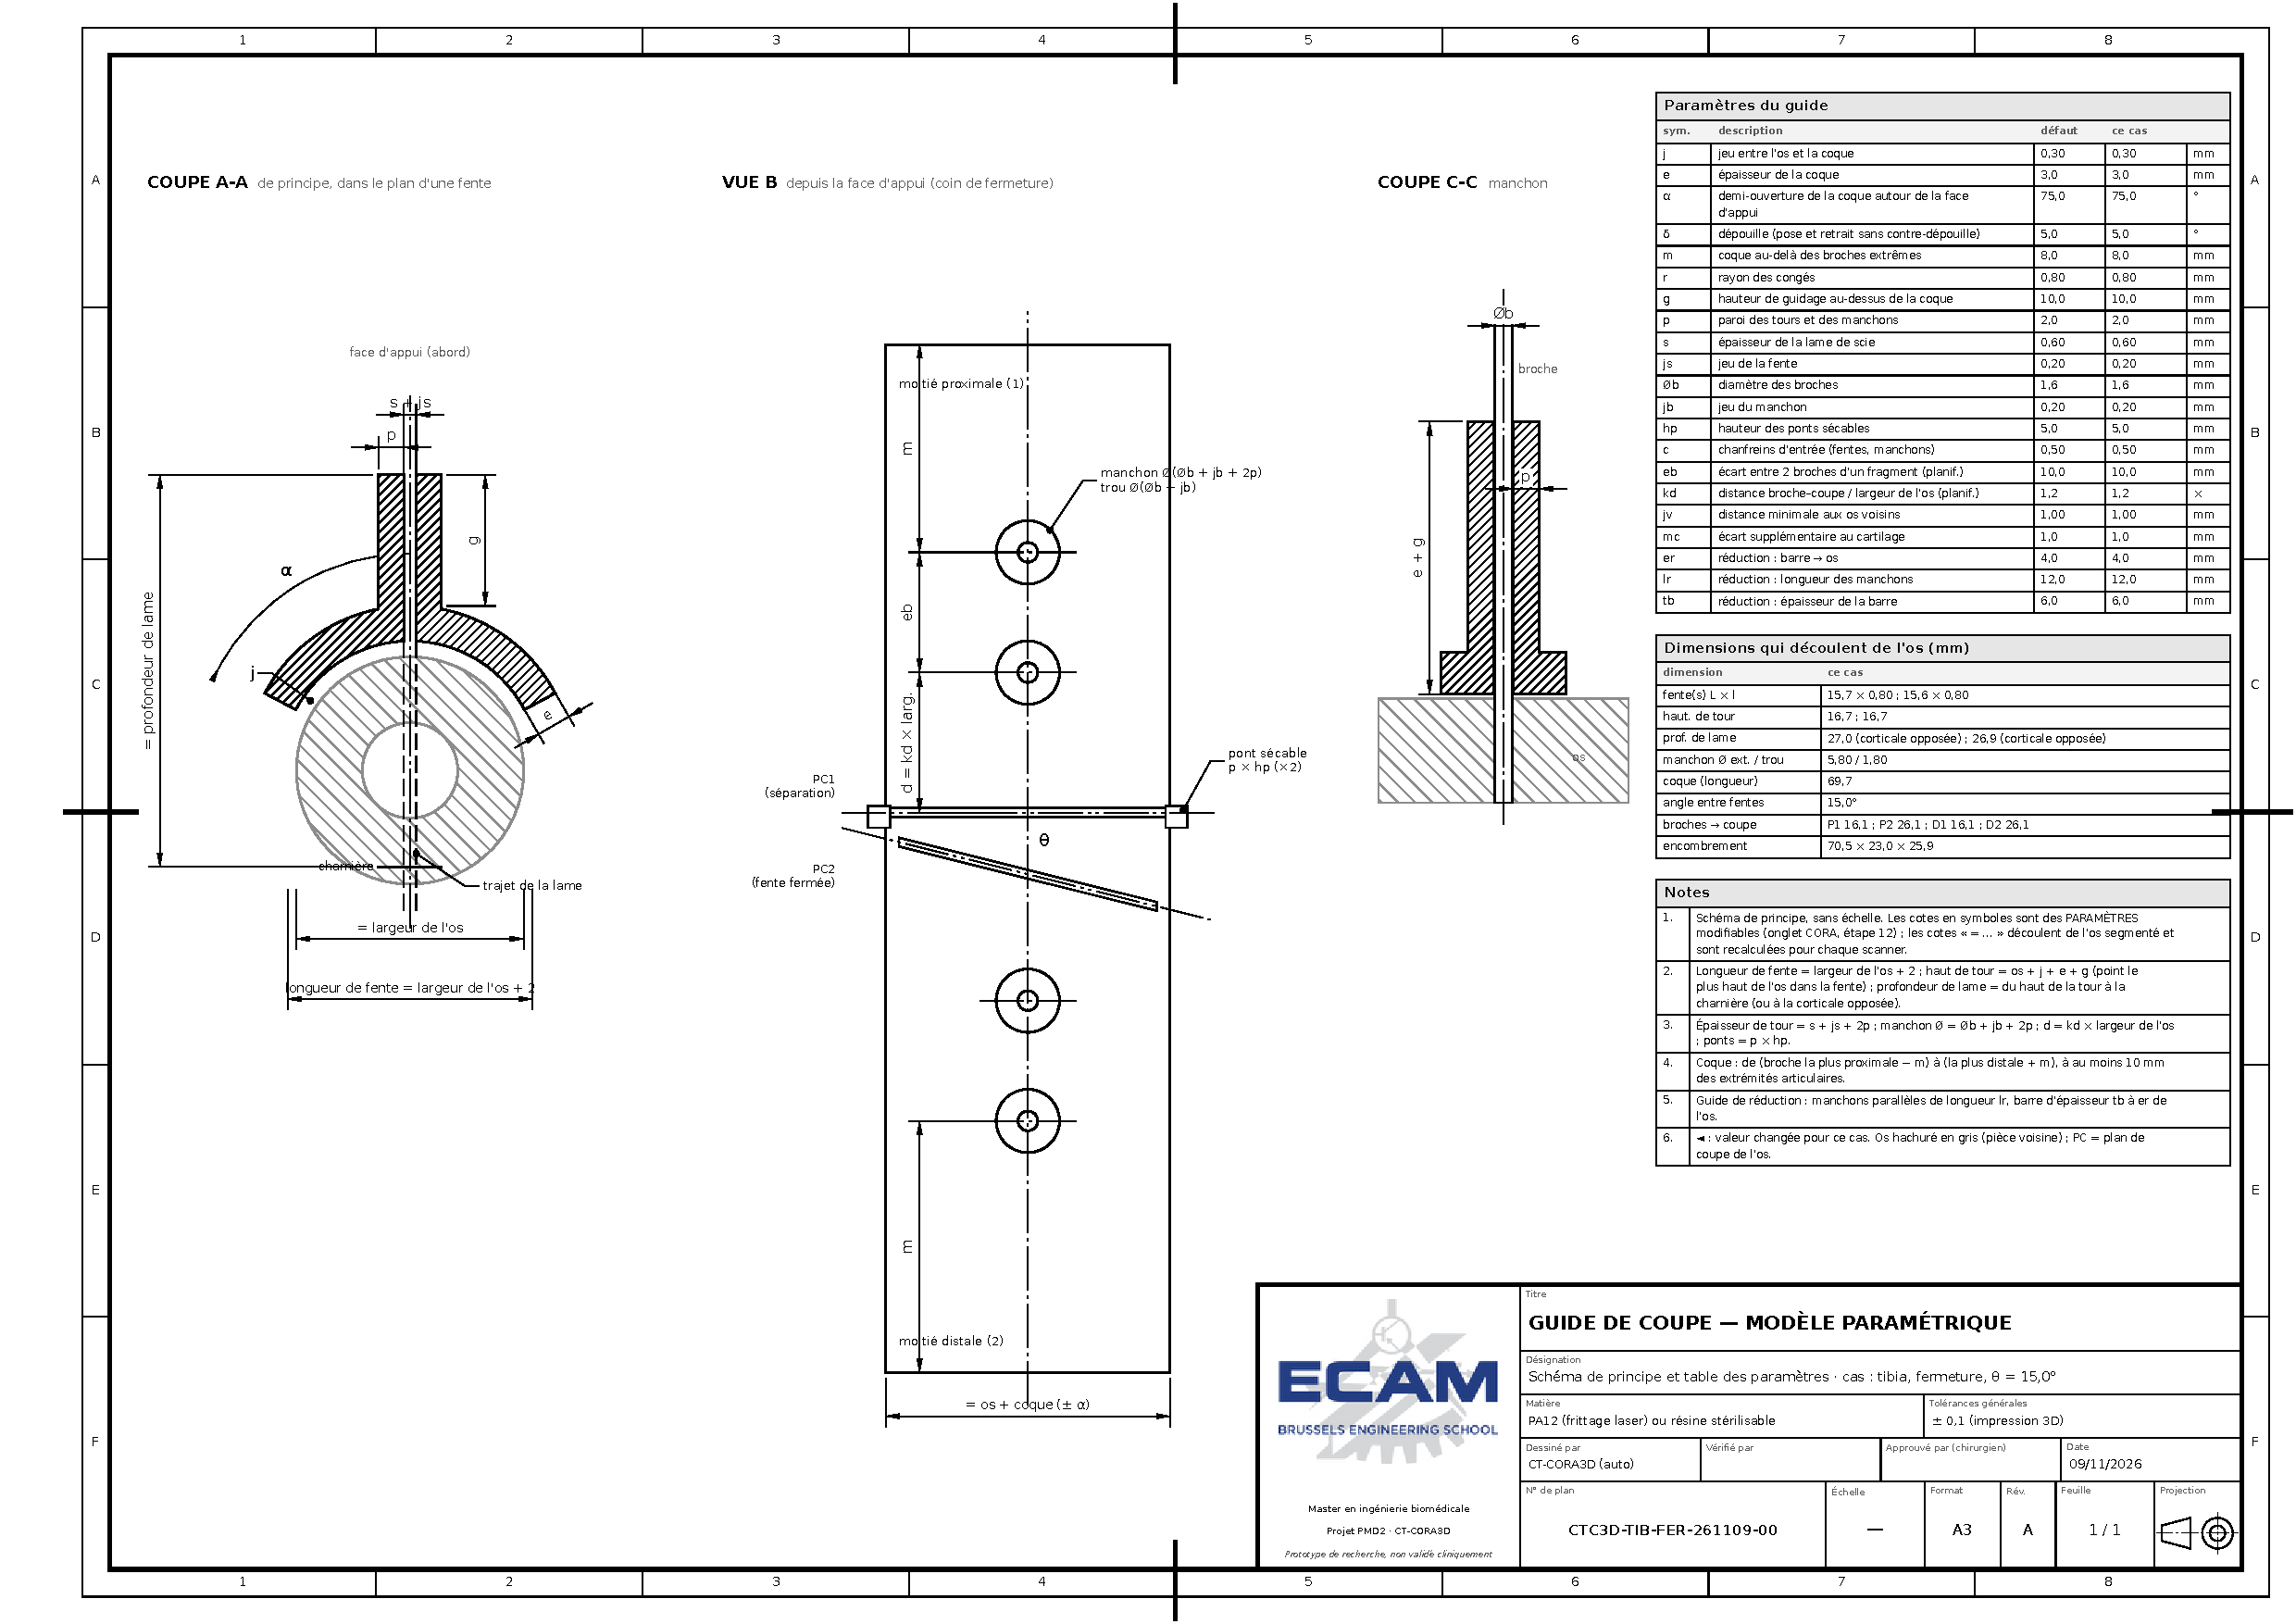
\includegraphics[width=\linewidth, height=0.9\textheight, keepaspectratio]{plan_generique.pdf}
\caption{Le plan générique du guide : le modèle paramétrique, avec ses cotes en symboles, le tableau des
paramètres et le cartouche (feuille A3 réduite ; le PDF est vectoriel, on peut zoomer).}
\label{fig:plan-generique}
\end{figure}
\begin{figure}[p]
\centering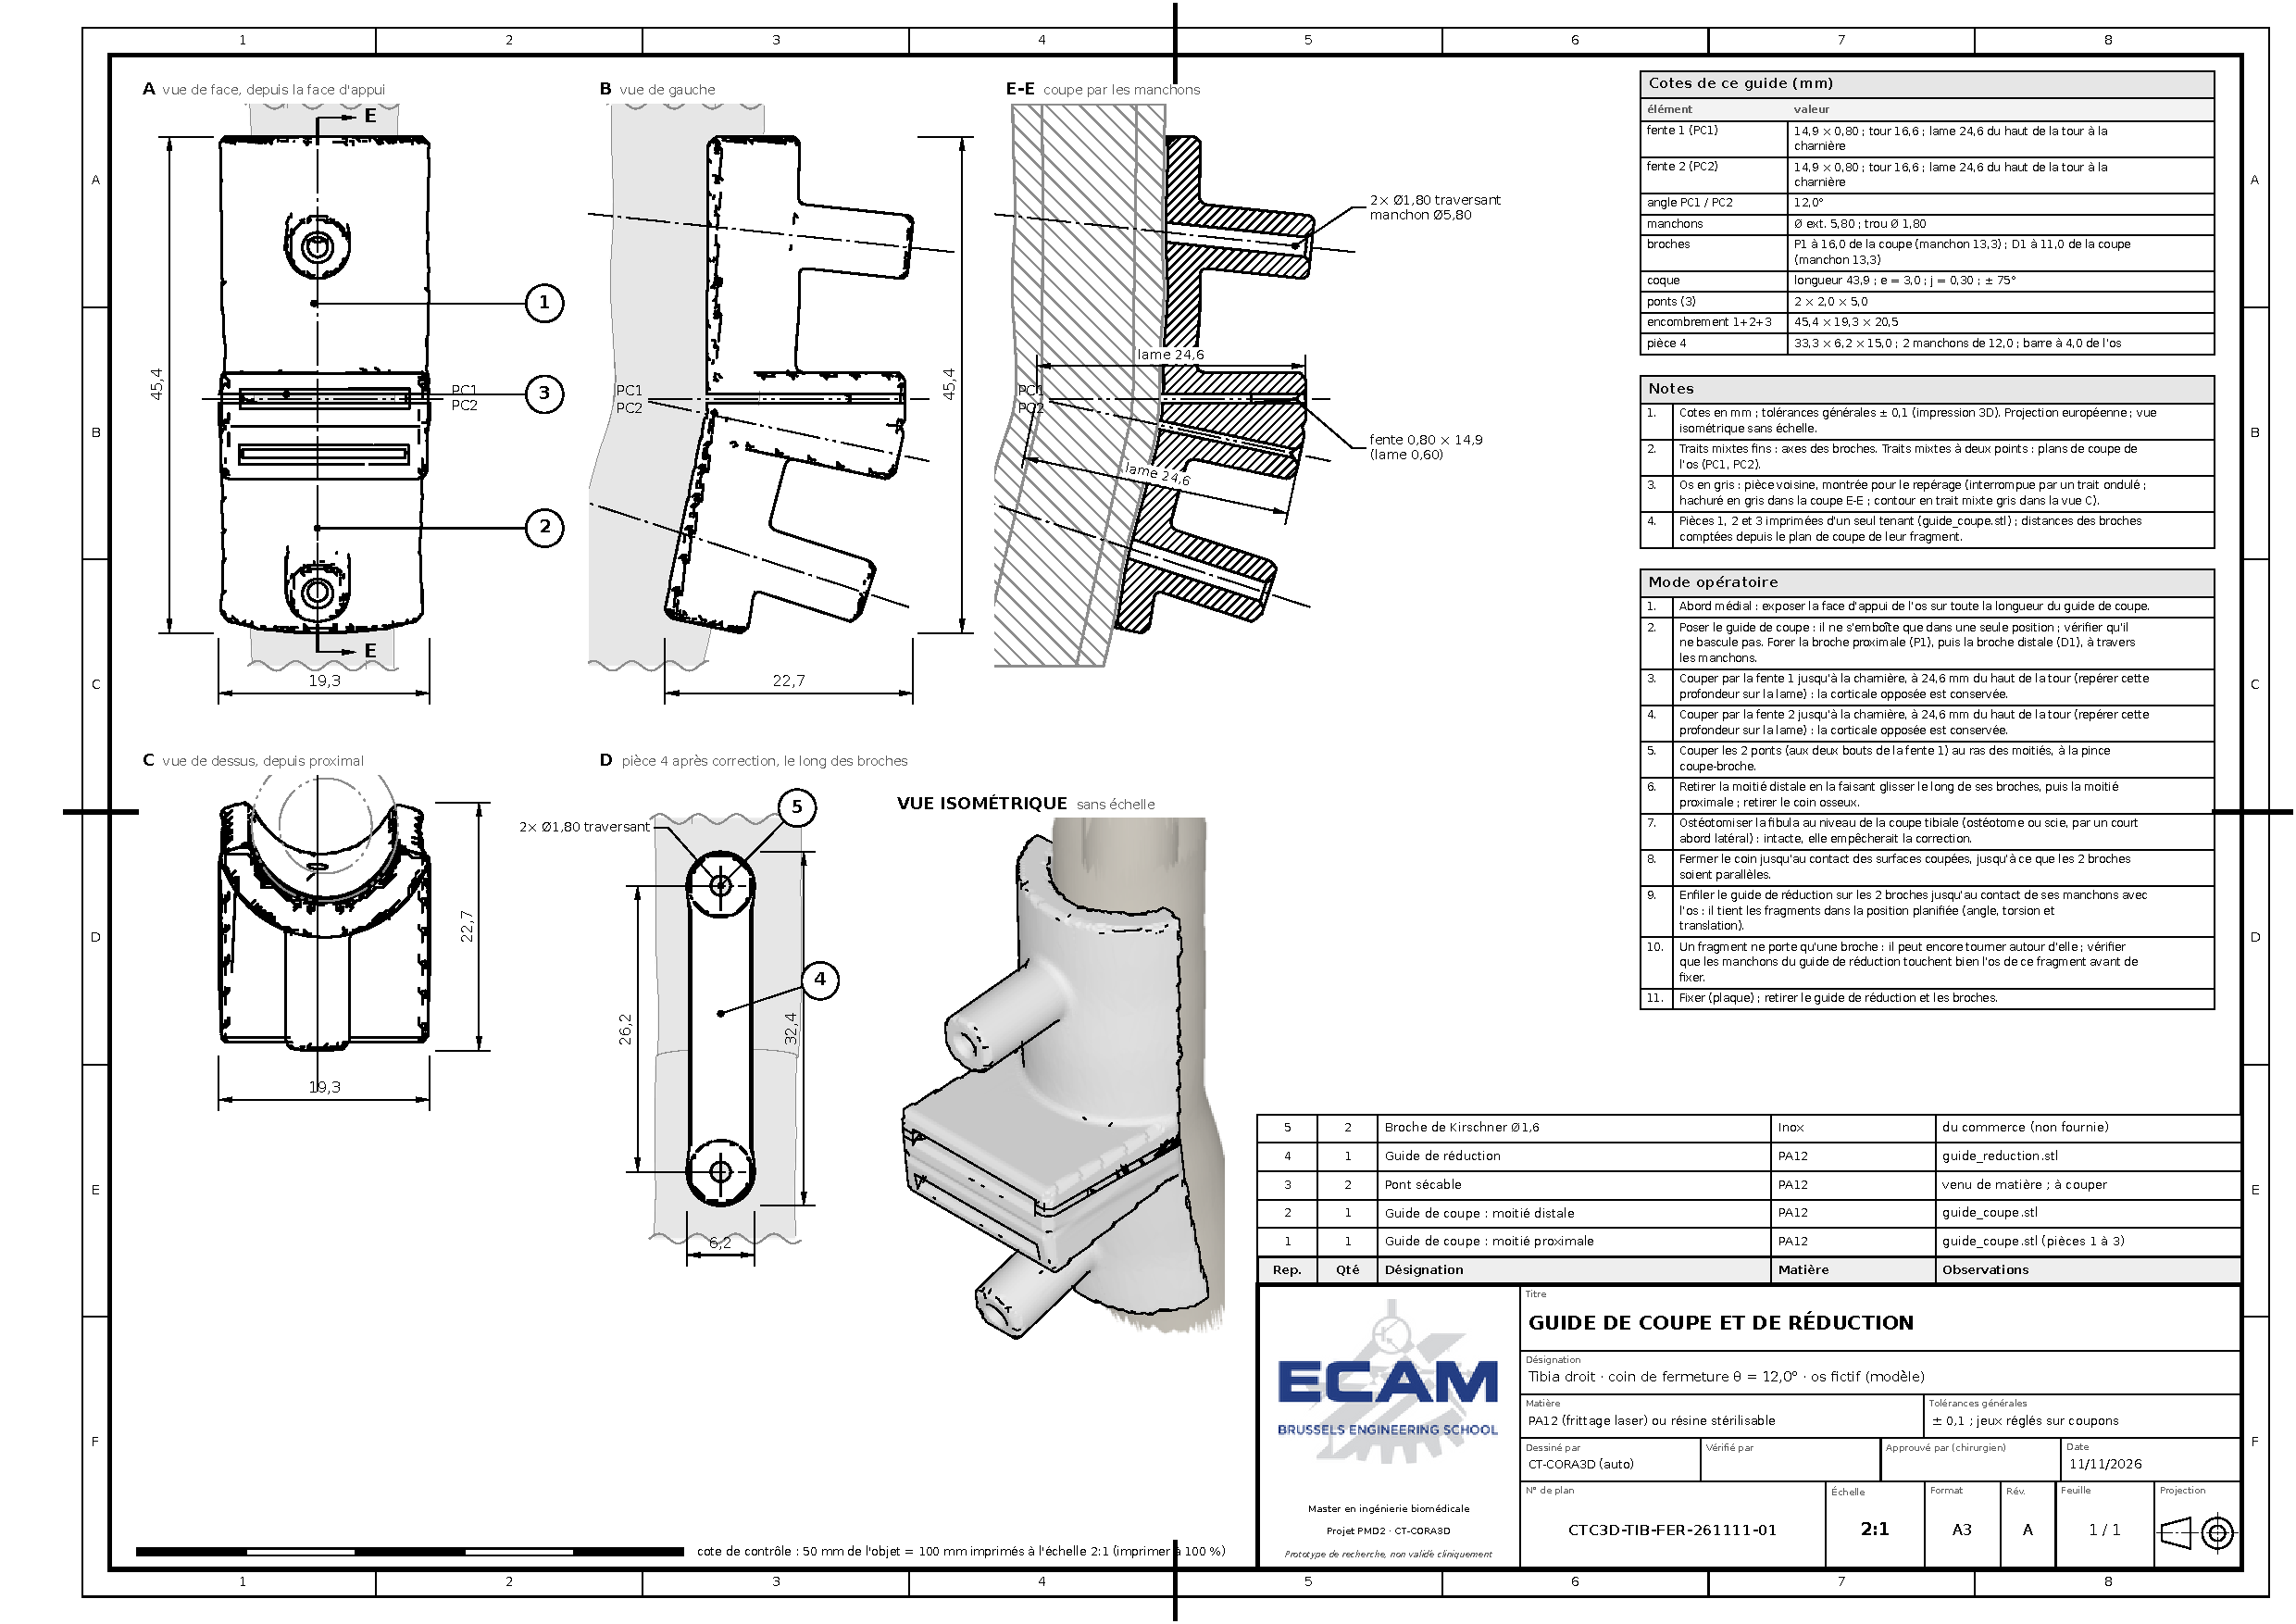
\includegraphics[width=\linewidth, height=0.9\textheight, keepaspectratio]{plan_guide.pdf}
\caption{Le plan coté produit automatiquement pour un guide de coin de fermeture du tibia : vues A, B et C,
coupe E-E, guide de réduction D, vue isométrique, nomenclature et cartouche (feuille A3 réduite).}
\label{fig:plan-guide}
\end{figure}
\end{landscape}
\pagestyle{fancy}
